\section{Configurable Sensor MAC ou CS-MAC}

O algoritmo desenvolvido nesse trabalho foi batizado de Configurable Sensor MAC ou Sensor-MAC configurável pois tem como base o algoritmo S-MAC descrito em \citeauthoronline{ye04} (\citeyear{ye04}). Conforme apresentado na sessão ~\ref{sec:smac}, o protocolo S-MAC faz com que cada nó em uma vizinhança siga um mesmo cronograma que determina seus períodos de atividade e inatividade. Com isso, cada nó que deseja transmitir pacotes poderá fazê-lo no momento em que iniciar seu ciclo de atividades sem a necessidade do uso de longos preâmbulos pois o nó receptor iniciará seu ciclo de atividades no mesmo momento.

O protocolo CS-MAC possui os mesmos mecanismos de funcionamento do protocolo S-MAC, podendo ser então considerado uma extensão desse protocolo, pois adiciona a ele mecanismos que permitem que seu funcionamento e configurações sejam alterados por outras camadas da pilha de protocolo, no caso do corrente trabalho, pela camada de aplicação (Sessão ~\ref{sec:applicationLayer}). 

Basicamente, os mecanismos de configuração implementados no protocolo CS-MAC permitem que outra camada possa determinar que o nó siga um cronograma de funcionamento arbitrário especificado por ela com qualquer finalidade. Para o teste dos mecanismos implementados no protocolo CS-MAC, foram implementados na camada de aplicação algoritmos capazes de construir uma ``via de acesso rápido'', por onde os pacotes poderiam trafegar mais rapidamente.

De forma simplificada, os algoritmos implementados são capazes de determinar que uma cadeia de nós situados a uma determinada distância do centro da rede (Figura ~\ref{fig:circularBackbone}) de sensores seja sincronizada de uma maneira tal que, dados os nós A, B e C pertencentes a estrutura, o tempo de transmissão de um pacote de A para C passando por B seria de aproximadamente $2 \cdot T_A$  ($1 \cdot T_A$ = transmissão de A para B, $1 \cdot T_A$ = transmissão B para C) sendo $T_A$ a duração do período de atividade de um nó. 

\begin{figure}[!htb]
\centering
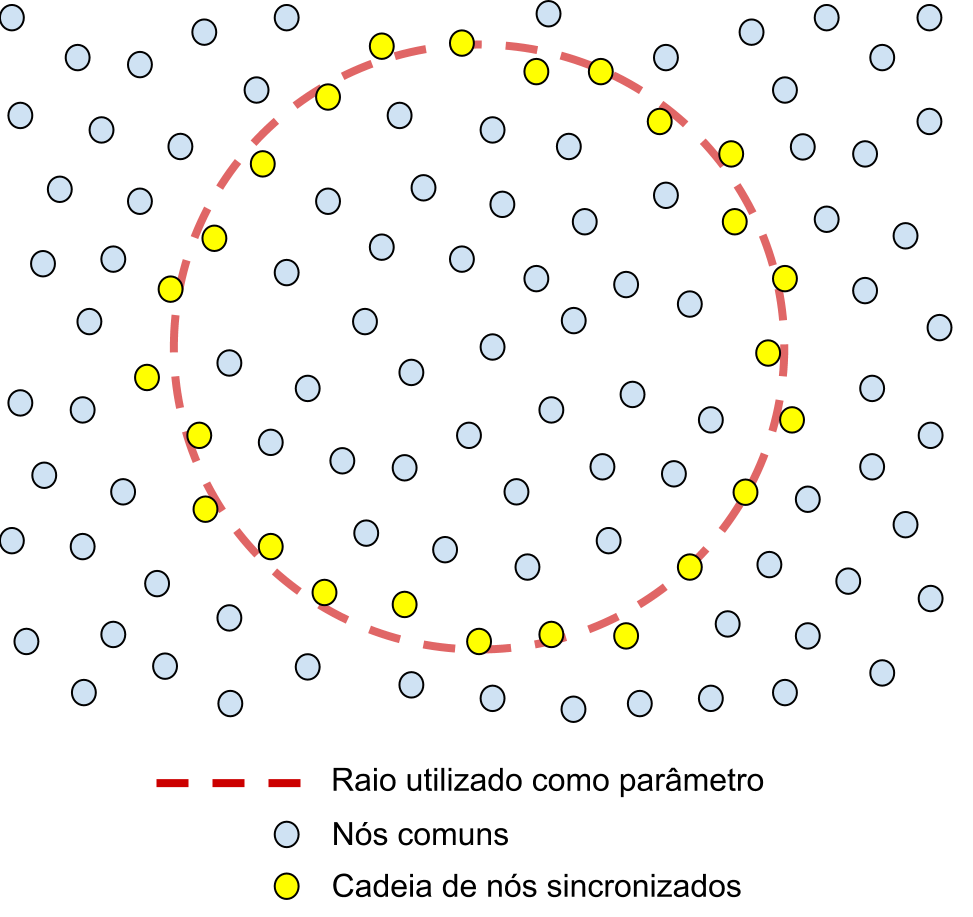
\includegraphics[width=297px,height=280px]{./Pictures/CircularBackbone.png}
% pdfLaTeX aceita figuras no formato PNG, JPG ou PDF
\caption{Cadeia de nós selecionados para sincronização} %legenda
\label{fig:circularBackbone} %rotulo para refencia
\end{figure}

Deve-se notar que não há intervalo entre as duas transmissões. Para que isso seja possível foi determinado que cada nó siga dois cronogramas de atividades distintos sendo que o primeiro cronograma determina um período de atividade no instante $X$ e o segundo determina um período de atividade no instante $X + T_A$. Além disso, primeiro ciclo de atividade de cada nó que participa da cadeia descrita acima deve coincidir com o segundo ciclo de atividades de seu antecessor. A figura ~\ref{fig:backboneSynchronization} abaixo mostra como estão sincronizados os nós do exemplo anterior.

\begin{figure}[!htb]
\centering
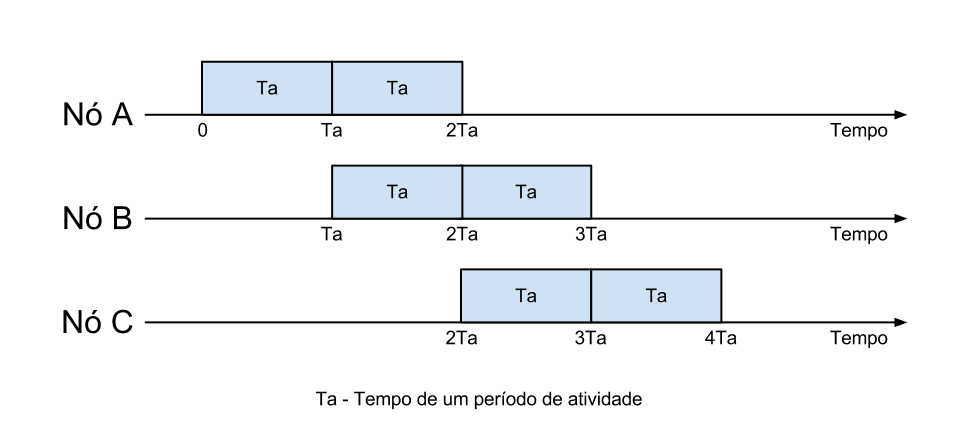
\includegraphics[width=350px,height=163px]{./Pictures/SequencialSynchronization.png}
% pdfLaTeX aceita figuras no formato PNG, JPG ou PDF
\caption{Cronogramas de atividade sincronizados sequencialmente} %legenda
\label{fig:backboneSynchronization} %rotulo para refencia
\end{figure}

As sessões seguintes apresentarão uma descrição mais pormenorizada dos algoritmos utilizados para produzir a organização descrita. Ao final serão também apresentados e discutidos os resultados de simulações realizadas para avaliação dos impactos dessa organização no tempo de transmissão de pacotes entre pontos distantes na rede de sensores.

\section{Algoritmos}

Esse capitulo apresentará os algoritmos utilizados para sincronização dos nós da rede, construção da  cadeia de nós que funcionará como via de transmissão rápida de pacotes e demais algoritmos utilizados. A sessão seguinte apresenta mais detalhes acerca do funcionamento do protocolo S-MAC (protocolo selecionado para a sincronização dos nós) e razões para a escolha do mesmo, bem como das alterações propostas para a construção do protocolo CS-MAC.

\subsection{Sincronização dos nós}

Como o objetivo do trabalho era o desenvolvimento de um protocolo de comunicação capaz de reduzir o tempo de transmissão de pacotes entre nós distantes na rede e ao mesmo tempo manter o consumo de energia no menor patamar possível, o protocolo S-MAC, citado anteriormente (Sessão ~\ref{sec:smac}) e encontrado em \citeauthoronline{ye04} (\citeyear{ye04}), foi selecionado como base para a construção do novo algoritmo. Esse algoritmo tem como foco o consumo reduzido de energia, além de possuir mecanismos eficientes para redução de perda de pacotes e solução de outros problemas inerentes às RSSFs, porém o tempo de transmissão entre nós distantes pode ser muito grande devido ao tamanho dos períodos de dormência dos nós em relação aos curtos períodos de atividade.

No protocolo S-MAC, cada nó possui pelo menos uma agenda que determina os momentos em que o rádio-transmissor do nó será ligado (quando o nó poderá enviar e receber pacotes) ou desligado. Essa agenda é compartilhada entre nós vizinhos, podendo haver regiões que possuam agendas distintas chamadas \emph{clusters} (Figura ~\ref{fig:SmacSynch}). Para que seja possível a comunicação entre essas regiões distintas, os nós que estejam no limiar dessas regiões compartilham ambas as agendas, dessa forma podendo enviar e receber pacotes para outros nós de ambas as regiões.

O mecanismo de criação e disseminação de agendas no protocolo S-MAC funciona de maneira auto organizada, não necessitando de interferência de agente externo. O novo protocolo desenvolvido nesse trabalho, assim chamado CS-MAC, propõe então uma extensão ao protocolo S-MAC de modo a disponibilizar mecanismos que permitam a configuração de agendas para os nós de maneira arbitrária por outras camadas da pilha de protocolos. Foi desenvolvido também nesse trabalho um algoritmo para a camada de aplicação que irá determinar, através desse mecanismo de configuração,  que certos nós sigam agendas específicas que farão com que possuam ciclos de atividade com intervalos muito pequenos entre si (Figura ~\ref{fig:backboneSynchronization}), de forma a construir uma cadeia de nós que acordem sequencialmente onde, consequentemente, a transmissão de pacotes por múltiplos nós ocorrerá de maneira muito mais rápida.

Para possibilitar um melhor entendimento do protocolo S-MAC e do protocolo proposto, a sessão seguinte irá apresentar mais detalhes do funcionamento de ambos.

\subsection{Funcionamento do protocolo S-MAC}

A partir do momento em que os nós que utilizam o protocolo S-MAC são ligados, eles realizam as seguintes operações:

\begin{itemize}
	\item ``Ouvir'' um ciclo inteiro esperando receber uma agenda que possa seguir.
	\item Caso não receba uma agenda, fará um teste utilizando um valor aleatório para determinar se criará sua própria agenda ou continuará a ``ouvir'' o meio por mais um ciclo.
	\item Tendo criado ou recebido uma agenda, irá configurar-se para acordar e dormir de acordo com essa agenda.
\end{itemize}

A partir do momento em que um nó adquire uma agenda seus ciclos de atividade e sono passarão a ser executados repetidamente. Alguns outros mecanismos fazem parte do protocolo, mas um aprofundamento maior foge ao escopo desse trabalho. Mais detalhes sobre o funcionamento do protocolo S-MAC podem ser encontrados em \citeauthoronline{ye04} \citeyear{ye04}. 

Além dos mecanismos providos pelo protocolo S-MAC, o novo algoritmo adiciona uma \emph{API} (\emph{Application Program Interface}) para que outras camadas da pilha de protocolo possam determinar novas agendas para o nó. Por meio desta, diferentes tipos de configurações para a sincronização entre os nós podem ser determinadas, por exemplo, pela camada de aplicação.

Nesse trabalho, o algoritmo desenvolvido utiliza agentes que percorrem a rede em busca de nós que cumpram determinados requisitos, de modo a formarem uma cadeia circular (Figura ~\ref{fig:circularBackbone}). Cada um dos nós selecionados é determinado pelo agentes a seguir duas novas agendas uma compartilhada com seu antecessor outra com seu sucessor na estrutura criada (Figura ~\ref{fig:backboneSynchronization}), sendo que essas agendas tem um intervalo muito pequeno entre si, suficiente para uma transmissão de pacotes entre os nós. Como resultado do trabalho dos agentes, os nós da cadeia circular estarão sincronizados sequencialmente. Transmissões de pacotes entre nós distantes na rede deverão percorrer essa estrutura visando reduzir o tempo total de transmissão do pacote do nó de origem ao nó destino. As sessões seguintes discutirão os algoritmos utilizados para configuração da rede e disseminação dos agentes.

\subsection{Cálculo da distância ao centro da rede}
\label{sec:calculoDistancia}

Para se determinar a distância de cada nó ao centro da rede é necessário conhecer a sua posição. A maneira mais simples é a utilização de nós que possuam sistema de \emph{GPS} (\emph{Global Positioning System} ou Sistema de Posicionamento Global). Tal sistema permite determinar com precisão a posição a posição de cada nó. Bastaria então que os agentes conhecessem as coordenadas de um ponto no centro da rede para que pudessem determinar se um nó satisfaz ou não os parâmetros que determinam o raio da estrutura circular a ser construída.

Para a utilização de sistema de posicionamento global (GPS) é necessário que cada nó possua \emph{hardware} específico para tal, o que aumenta o seu custo e consumo de energia. Como alternativa ao uso desse sistema é possível realizar o cálculo das distâncias a partir de um nó central. Esse nó inicial comunicaria em \emph{broadcast} aos seus vizinhos que ele é o ponto zero. Cada um de seus vizinhos que receba esse pacote poderá determinar sua distância a esse nó central com base na intensidade do sinal recebido.  Cada um desses nós então irá fazer um novo \emph{broadcast} para informar sua distância do centro e assim sucessivamente. 

Para aumentar a precisão do cálculo de sua posição, um nó que já tenha recebido um desses pacotes e receba um novo pacote que determine uma distância menor ao centro da rede, atualizará seu parâmetro de distância e fará um novo \emph{broadcast} para atualizar seus vizinhos. Isso irá gerar um \emph{flooding} de pacotes na rede, após o qual cada nó conhecerá sua posição e a de seus vizinhos em relação ao nó central e os agentes poderão utilizar esses valores para a construção da estrutura circular. 

\subsection{Construção do círculo}
\label{sec:circleBuilding}

Dado que a distância de cada nó em relação ao centro da rede pode ser obtida através das soluções apresentadas na sessão anterior (~\ref{sec:calculoDistancia}), foram utilizados três agentes para a construção da estrutura circular: 

\begin{itemize}
 \item \textbf{\emph{Root finder:}} responsável por percorrer a rede em busca de algum nó que cumpra o requisito de distância do centro da rede (raio do circulo formado). O nó selecionado por esse agente será o nó raiz na estrutura a ser formada. Após encontrar o nó raiz, esse agente irá criar o próximo agente. 
 \item \textbf{\emph{Circle builder:}} responsável por criar as agendas para cada nó (incluindo o nó raiz), determinar qual vai ser o próximo nó que fará parte da estrutura. Ele selecionará vários nós (conforme os mesmos parâmetros do nó anterior) até alcançar algum que já faça parte da estrutura (fechando o círculo), quando então ele criará o próximo agente.
 \item \textbf{\emph{Circle revoker:}} caso o último nó encontrado pelo agente \emph{Circle builder} não coincida com o nó raiz encontrado pelo agente \emph{Root finder}, esse agente será responsável por remover as agendas extras dos nós que foram selecionado, mas não fazem parte do círculo formado (``pontas soltas''), fazendo com que eles voltem a seguir apenas suas agendas originais.
\end{itemize}

\subsection{Roteamento dos pacotes}

Para que a configuração circular formada dentro da rede pelos algoritmos descritos nas sessões anteriores produza efeitos sobre o tempo das transmissões de pacotes dentro da rede, é preciso rotear os pacotes de forma que, caso seja possível, eles sejam encaminhados através da estrutura formada até um ponto próximo do nó destino, quando o pacote deixará a estrutura e será encaminhado ao seu destino através dos mecanismos normais. 

A elaboração de um algoritmo de roteamento de pacotes foge ao escopo desse trabalho. Portanto, com o objetivo de avaliar o desempenho do algoritmo proposto, a determinação do nó receptor em cada transmissão foi feita pelo gerenciador da simulação conforme os seguintes critérios:

\begin{itemize}
\item Caso haja um nó vizinho ao nó transmissor que pertencente à estrutura formada e que esteja mais próximo do nó de destino do pacote do que o transmissor, esse nó será selecionado
\item Caso o critério anterior não seja cumprido, será selecionado como receptor, aleatoriamente, um dos três nós vizinhos mais próximos do nó de destino
\end{itemize}

Utilizando esses critérios foi possível simular um algoritmo de roteamento capaz de fazer com que os pacotes sejam transmitidos através da estrutura circular formada, possibilitando assim a avaliação de seu desempenho.



